\section{Results}

In the following the performance of I2A over the model-free baseline and the copy model is shown. Also the predicted rollouts of the environment model.

\subsection{Environment Model Training}

The trained environment model is a imperfect model which is in most cases able to predict a few steps into the future, but it is bad in predicting far into the future.\\

The figrue \ref{fig:env_model_loss} show the loss curve of the environment model training. It seems as if the loss stagnates very soon, but the main advantage in correct predictions is learned in the part with small loss changes. To learn the general structure of the maze is easy but to predict the correct position of the player and the ghosts is really hard.

TODO loss curve
\begin{figure}[H] 
  \centering   
  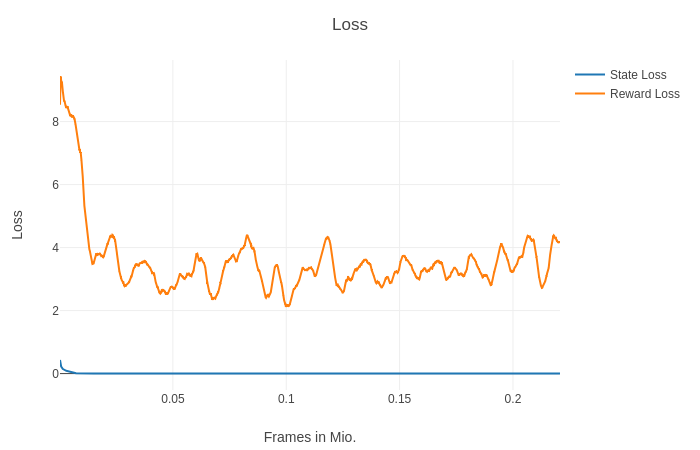
\includegraphics[width=0.9\columnwidth]{./Images/hunt_environment_model_loss.png}
  \caption{Environment model loss curve} 
  \label{fig:env_model_loss} 
\end{figure} 


Figure \ref{fig:environment_model_rollouts} shows the true next observation in the upper row and the predicted observation in the lower row. From left to right it shows the rollout steps, the prediction is always based on the previouse rollout step. In the beginning the prediction is quite good but the errors accumulate, leading to prediction errors like the one in rollout step 3 of figure \ref{fig:environment_model_rollouts}. The environment model is unsure where the ghost, the red points, are moving and as a result it predicts the ghost at two positions.

\begin{figure}[H] 
  \centering   
  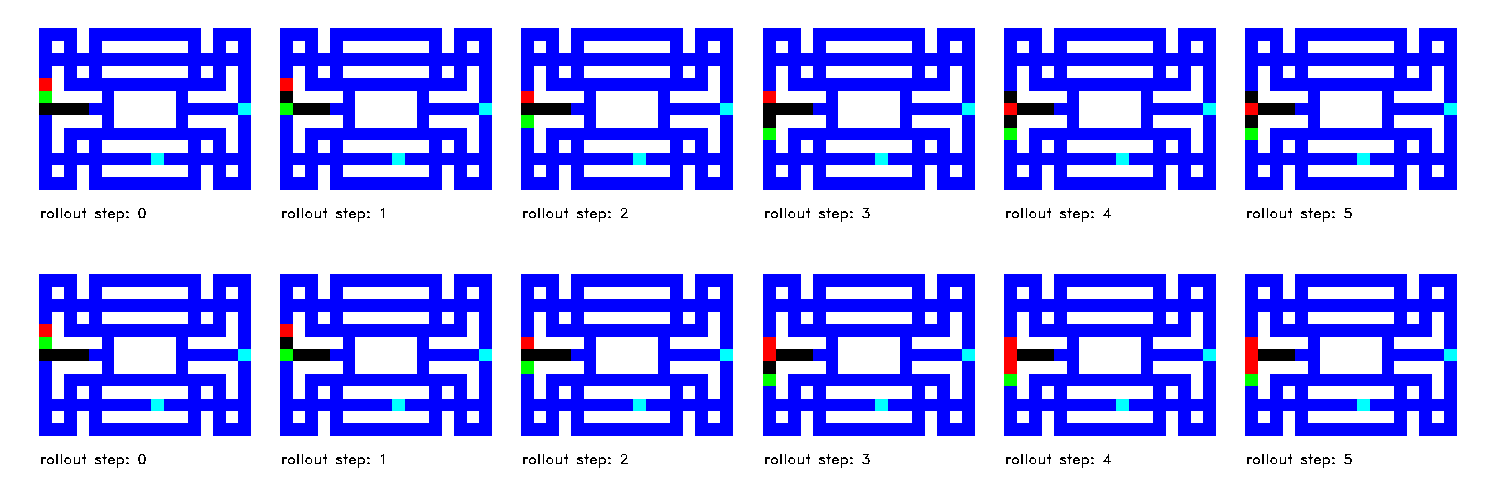
\includegraphics[width=\columnwidth]{./Images/env_model_rollouts.png}
  \caption{Environment model rollouts, top true observation, bottom predicted observation, rollouts steps from left to right} 
  \label{fig:environment_model_rollouts} 
\end{figure} 



\subsection{I2A MiniPacman Results}

TODO regular results.\\

To compare the performance, we trained MiniPacman Hunt with a A2C model-free baseline, the copy model and I2A agent. The results are shown in figure \ref{fig:mini_pacman_hunt_rewards}. As you can see the I2A algorithm outperformce A2C and the Copy model.


\begin{figure}[H] 
  \centering   
  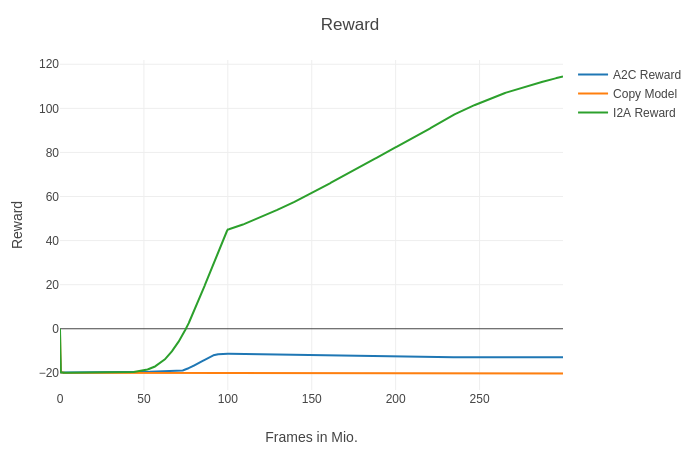
\includegraphics[width=0.9\columnwidth]{./Images/hunt_rewards_compare.png}
  \caption{A2C Hunt Reward Training Curve (100 mio frames)} 
  \label{fig:mini_pacman_hunt_rewards} 
\end{figure} 
